\documentclass[a4paper,12pt]{article}
\usepackage{amsmath,amssymb}
\usepackage{enumerate}
\usepackage{enumitem}
\usepackage{graphicx}
\usepackage{ wasysym }
\usepackage{pythonhighlight}


\newcommand{\given}{\,|\,}
\newcommand{\R}{\mathbb{R}}
\newcommand{\E}{\mathbb{E}}
\newcommand{\var}{\text{var}}
\newcommand{\cov}{\text{cov}}
\newcommand{\trans}{\mathsf{T}}
\newcommand{\bx}{\mathbf{x}}
\newcommand{\by}{\mathbf{y}}
\newcommand{\bw}{\mathbf{w}}
\newcommand{\distNorm}{\mathcal{N}}
\newcommand{\bzero}{\mathbf{0}}
\newcommand{\ident}{\mathbb{I}}
\newcommand{\N}{\mathcal{N}}
\newcommand{\ep}{\varepsilon}
\newcommand{\norm}[1]{\left\lVert#1\right\rVert}

\title{CSC410 A5}
\author{Joshua Prier, }

\begin{document}
	\maketitle
	
	\begin{enumerate}
		\item 
			\begin{enumerate}
				\item \textbf{All Paths:}\\
				1,2,3,9,10,11\\
				1,2,3,9,13,14\\
				1,5,6,7,9,10,11\\
				1,5,6,7,9,13,14\\
				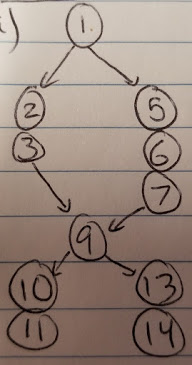
\includegraphics[scale=.5]{q1graph.jpg}
				\item 
					\begin{tabular}{|c|c|c|}
						\hline
						\multicolumn{3}{|c|}{Infeasible Path} \\
						\hline
						Line No. & Assignment & Path Conditions \\
						\hline
						1,2,3   & $x\leftarrow X-5$ & $X+Y > 10$ \\
						  ~ & $y\leftarrow Y+5$ & ~   \\
						\hline
						9,10,11  & $x\leftarrow -(X-5)$ & $X+Y > 10$ \\
						~ & $y\leftarrow -(Y+5)$ & AND $ (X-5) + (Y+5) < 0$   \\
						\hline
					\end{tabular} ~\\\\
				This path is infeasible because of the conflicting path conditions. $10 < (X+Y) = (X-5) + (Y+5) \nless 0$.
				\item 	\begin{tabular}{|c|c|c|}
					\hline
					\multicolumn{3}{|c|}{Assertion Violation Path} \\
					\hline
					Line No. & Assignment & Path Conditions \\
					\hline
					1,5,6,7   & $x\leftarrow Y$ & $X+Y \le
					 10$ \\
					~ & $y\leftarrow X$ & ~   \\
					\hline
					9,13,14  & $x\leftarrow Y-1$ & $X+Y \le 10$ \\
					~ & $y\leftarrow X-1$ & AND $ X + Y \ge 0$   \\
					\hline
				\end{tabular} ~\\\\
			This path will cause an assertion violation in the case that $X+Y \le 2$ since the assignments from 9,13,14 subtract 2 from the sum, $(X-1) + (Y-1) = X + Y - 2$\\\\
			
			\textbf{Why the other 2 paths never cause an assertion violation:}\\
			\begin{tabular}{|c|c|c|}
				\hline
				\multicolumn{3}{|c|}{Assertion Violation Path} \\
				\hline
				Line No. & Assignment & Path Conditions \\
				\hline
				1,5,6,7   & $x\leftarrow Y$ & $X+Y \le
				10$ \\
				~ & $y\leftarrow X$ & ~   \\
				\hline
				9,10,11  & $x\leftarrow -Y$ & $X+Y \le 10$ \\
				~ & $y\leftarrow -X$ & AND $ X + Y < 0$   \\
				\hline
			\end{tabular} ~\\\\
			Since  $x\leftarrow -Y$ and $y\leftarrow -X$ and $X+Y<0$ then $(X-1) + (Y-1) = -(X+Y) > 0$
		
			\begin{tabular}{|c|c|c|}
				\hline
				\multicolumn{3}{|c|}{Assertion Violation Path} \\
				\hline
				Line No. & Assignment & Path Conditions \\
				\hline
				1,2,3   & $x\leftarrow X-5$ & $X+Y >
				10$ \\
				~ & $y\leftarrow Y+5$ & ~   \\
				\hline
				9,13,14  & $x\leftarrow (X-5)-1=X-6$ & $X+Y > 10$ \\
				~ & $y\leftarrow (Y+5)-1=Y+4$ & AND $ X + Y \ge 0$   \\
				\hline
			\end{tabular} ~\\\\
			Since $X+Y>10$ then $(X-6) + (Y+4) = X+Y-2 > 10-2 = 8$ therefore $x+y > 0$
		
			\end{enumerate}
		\item \begin{enumerate}
			\item $\square b \rightarrow b \cup o$
			\item $\square \neg o \rightarrow ((r \rightarrow \ocircle w) \wedge (w \rightarrow \ocircle r)$
			\item $\square \neg o \rightarrow r \cup (b \cup (w \cup r))$
			\item $\square (r \wedge b \wedge g) \rightarrow \ocircle w$
			\item $\square r \rightarrow r \cup \neg r$
		\end{enumerate}
		\item 
		\item 
		\item 
		\item 
		\item 
		
		\textbf{Algorithm Explanation:}\\
		
		The algorithm that we have implemented finds the winning player by setting winning states on a grid of size m by n\\
		
		It starts at (0,0) the final state and sets it as the final state. Then we set all winning states that can get to the final state in one move. This means we fill the vertical (0,y), horizontal (x,0), and the diagonal (x,y) as winning states.\\
		
		In the next step we can check the lowest index of an empty/unset location on the grid, we then check if this state is a winning state. A winning state is a state that can reach the final state or put the other player in a loss state. A loss state is a state where all moves put the other player in a winning state. Then the current position's state is set, if the current state is a loss state we do the same as the final state and set all possible moves to get to that location as a winning state.\\
		
		This is repeated until the location (m,n) on the grid is filled\\
		
		\textbf{Code and Runtime:}\\
		
		The runtime complexity of the algorithm is roughly $O(\frac{m+n}{2})$ or under. This complexity runs any game within 100x100 games in well under a second. \\
		
		These times are done by looping through each row and only checking empty states in the grid, along with ending the algorithm as soon as the (m,n) state is found \\
		
		Additional time was gained through avoiding clean readable code and optimizing runtime, in python this means the code looks childish\\
		
		
		Here is the code, it uses all builtin python3 so no external packages are needed to run this.\\
		Code is also provided as a .py file on markus\\
		
		\begin{python}
		import sys
		import timeit
		from itertools import repeat
		
		
		def get_winning_player(m, n):
			# repeat avoids unnecessary i's being created
			grid = [['E' for i in repeat(None, m+1)] for j in repeat(None, n+1)]
			grid = set_grid_loses(grid, 0, 0, m, n) #(0,0) is a known state and can be set
			i = 0
			while i <= n:
				# quit once result is found -- Can delete if this is against the rules
				if grid[n][m] != 'E':
					return 1 if grid[n][m] == 'w' else 2
			
				while 'E' in grid[i]:
					j = grid[i].index('E')
					if is_winning_state(grid, i, j):
						grid[i][j] = 'w'
					else:
						grid = set_grid_loses(grid, i, j, m, n)
				i+=1
			
			return 1 if grid[n][m] == 'w' else 2
		\end{python}
	
		\begin{python}
		# if there is a move in which you can make the other player lose you are in a winning state
		def is_winning_state(grid, x, y):
			if 'l' in grid[x][:y]:
				return True
			for i in range(x):
				if grid[i][y] == 'l':
					return True
			for i in range(min(x, y)-1):
				if grid[x-i-1][y-i-1] == 'l':
					return True
			return False
		\end{python}~\\
	
		\begin{python}
		def set_grid_loses(grid, x, y, m, n):
			# (0,0) is an exception to the rules as it is the final state
			grid[x] = ['w'] * len(grid[x])
			for i in range(n+1):
				grid[i][y] = 'w'
				if i <= m:
					grid[i][i] = 'w'
			grid[x][y] = 'w' if x == 0 and y == 0 else 'l'
			return grid
		\end{python}
	
		\begin{python}
		def main():
			start = timeit.default_timer()
			m, n = int(sys.argv[1]), int(sys.argv[2])
			print("The winning player for game ({},{}) is: {}".format(m, n, get_winning_player(m,n)))
			stop = timeit.default_timer()
			print("Algo took: " + str(stop-start))
		
		
		if __name__ == "__main__":
			main()
		\end{python}
		
	\end{enumerate}
	
\end{document}